\section{Zusammensetzung des Ursprungsdatensatzes} \label{sec:Meth Datensatz}
\Gls{ML} benötigt Daten, um aus diesen allgemein gültige Informationen über eine Aufgabe zu extrahieren. Da die Vorauswahl der Modelle (\autoref{sec:Meth Nutzwert}) deutlich macht, dass Ansätze des überwachten Lernens verfolgt werden, wird auch ein \gls{Labelvektor} benötigt. Wie Ereignisse gelabelt und verifiziert werden, ist in \autoref{sec:Meth Labeling} erläutert. In diesem Abschnitt wird erläutert wie sich der Ursprungsdatensatz, aus dem später der Trainingsdatensatz und der Testdatensatz hervorgehen, zusammensetzt. Dargestellt wird Wie die Mengenverhältnisse von Kontrollgangereignissen, Kampfereignissen und Normalverhalten sind und die Datenmenge wird diskutiert in Bezug auf die Erfolgsaussichten. 

\subsection{Heraussuchen der Ereignisse}
Wie in \autoref{sec:Meth Labeling} erwähnt, steht für die Verifizierung ein Datensatz mit Ereignissen zur Verfügen. Dieser beinhaltet Ereignisse von allen drei Verhaltensweisen. Die Tabelle \ref{tab:bspUnvDataSet} zeigt den Aufbau dieses Datensatzes exemplarisch. 


\begin{table}[ht]
    \centering
    \caption{Beispielhafter Auszug aus dem Ereignisdatensatz vor der Verifikation.}
    \begin{tabular}{|c|c|c|c|}
        \hline
        Startzeit & Endzeit & KameraID & Label\\
        \hline
        05.05.2021 13:57:00 & 05.05.2021 13:59:00 & 3       & Kampf\\
        \hline
        11.05.2021 06:13:21 & 11.05.2021 06:14:51 & 5       & Kontrollgang\\
        \hline
        \vdots              & \vdots              & \vdots  & \vdots\\
        \hline
        13.06.2021 19:00:03 & 13.06.2021 19:04:17 & 5       & Normalverhalten\\
        \hline
    \end{tabular}
    \label{tab:bspUnvDataSet}
\end{table}

Das heraussuchen der Kampfereignisse erfolgte Manuell und bereits vor dieser Arbeit. Die Videos wurden angesehen und wenn ein Kampf festzustellen war, wurde über die Laufdauer des Videos die Uhrzeiten geschätzt, zu welchen der Kampf stattgefunden hat. Bei einer Untersuchung hat sich herausgestellt, dass die Schätzungen nur grob sind, Die Zeitpunktangaben sind ungefähr auf einen Zeitraum von 10 Minuten eingegrenzt. Die Zeitpuntke der Kontrollgänge wurden während der Mastdurchläufe aufgezeichnet. Beim betreten und verlassen des Stalls des Tierhalters wurden die Zeitstempel tabellarisch erfasst. Diese sind relativ genau. Die Zeitpunkte des Normalverhaltens wurden zufällig generiert. Da das was in dieser Arbeit als Normalverhalten deklariert ist, den Großteil der Zeit ausmacht, war zu vermuten, das mit diesem Vorgehen relativ zuverlässig Normalverhlaten markiert wird. Da bei der Generierung der Zeitpunkte die Verifizierung bereits geplant war, war bekannt, dass die Zufälligen Zeitpunkt überprüft werden. Die Zeitpunkte des Normalverhaltens wurden Gleichverteilt über den gesamten Mastdurchlauf generiert.\par

Die herausgesuchten Ereignisse entstammen alle dem ersten Mastdurchlauf. Da die manuelle Suche nach Kämpfen sehr zeitintensiv ist, war es im Rahmen dieser Arbeit nicht möglich, weitere Kämpfe herauszusuchen. Die Kämpfe die zuvor herausgesucht wurden entstammen alle dem ersten Mastdurchlauf. Genauer eingegrenzt sind Kämpfe auch nur aus dem Bildmaterial der Kameras mit den IDs 3 und 5 herausgesucht worden. Aus diesem Grund wurde sich im Aufbau des Modells auf diesen Mastdurchlauf und die Stallbereiche konzentriert, die von den Kameras Nummer 3 und 5 abgedeckt sind. Der erste Mastdurchlauf ging vom 14.03.2021 bis zum 18.06.2021, wobei die Aufzeichnungen erst zum 22.03.2021 begannen. \todo{Daten Checken} Die Zusammensetzung des Datensatzes dieser herausgesuchten Ereignisse ist in der Tabelle \ref{tab:DataSetUnVeri} zusehen.\par


\begin{table}[ht]
    \centering
    \caption{Zusammensetzung des Datensatzes der unverifizierten Ereignisse.}
    \begin{tabular}{|l|r|r|}
    \hline
        Verhaltensweise & Anzahl & Anteil \\
    \hline
        Normalverhalten & 160 & 30 \%\\
        Kontrollgang & 159 & 30 \%\\
        Kampf & 216 & 40 \%\\
    \hline
    \hline
        Gesamt & 535 & 100 \%\\
    \hline
    \end{tabular}
    \label{tab:DataSetUnVeri}
\end{table}


\subsection{Verifizierung der Ereignisse und Analysen}
Mittels des Programms zu Verifizierung der Ereignisse lässt sich ein Datensatz erzeugen, in welchem die Ereignisse zeitlich möglichst exakt eingegrenzt sind. Auch wird bekannt, welche Ereignisse sich nicht Verifizieren lassen, weil sie entweder nicht gefunden wurden, oder weil keine Detektionsdaten oder Videos zu ihnen vorhanden waren. Dabei ist aufgefallen, dass vor dem 14.04.2021 die Aufzeichnung stark fehlervehaft verlief. Videostream sind nicht vorhanden, oder unvollständig und die Detektionsdatensetze weisen zeitliche Lücken auf. Somit sind alle Ereignisse vor dem 14.04.2021 nicht verifizierbar. \par

Bei der Verifizierung der Kontrollgänge viel auf, dass sich diese oft in mehrere Phasen aufteilen. Neben den charakteristischen Merkmalen die in \autoref{sec:Meth DefAufgabe} beschrieben sind, kehrt zwischen diesen Merkmalen immer wieder Normalverhalten ein. Bezogen auf dem Datensatz bedeutet dies, aus einem Kontrollgangereignis lassen sich oft mehrere Phasen extrahieren in denen die  charakteristischen Merkmale auftreten. Die Tabelle \ref{tab:DataSetVeri} zeigt die Zusammensetzung des Datensatzes nach der Verifizierung, sowie die Veränderung zum Datensatz in \autoref{tab:DataSetUnVeri}. 

\begin{table}[ht]
    \centering
    \caption{Zusammensetzung des Datensatzes nach der Verifizierung.}
    \begin{tabular}{|l|r|r|r|}
    \hline
        Verhaltensweise & Anzahl & Anteil & Veränderung\\
    \hline
        Normalverhalten & 103 & 21 \% & -36 \%\\
        Kontrollgang & 188 & 39 \% & +18 \%\\
        Kampf & 196 & 40 \% & -9 \%\\
    \hline
    \hline
        Gesamt & 487 & 100 \% & -9 \% \\
    \hline
    \end{tabular}
    \label{tab:DataSetVeri}
\end{table}

Insgesamt sorgt die Verifizierung dafür, dass die Gesamtanzahl der Ereignisse schrumpft. Durch die Aufteilung der Phasen der Kontrollgänge ist ein Zuwachs der Kontrollgangereignisse festzustellen. Von Interesse ist auch, die Dauer der Ereignisse. Gerade die Kontrollgänge und Kämpfe zeigen zeitlich eine Begrenzung, während das Normalverhalten eher als der Normalzustand betrachtet wird, welcher von einem Kampf oder Kontrollgang unterbrochen wird. Dadurch besitzt Normalverhalten keinen klar definierten Start- und Endpunkt. bei der Verifizierung ist der Start- und Endpunkt vom Normalverhalten also eher so zu interpretieren, dass sichergestellt wird, dass sich in diesem Zeitraum kein Kampf und kein Kontrollgang abspielt.In der Abbildungen \ref{fig:EreignisDauer} sind die Unterschiedlichen Längen der Ereignisse in Histogrammen dargestellt.

\begin{figure}[htbp]
    \centering
    \begin{subfigure}{.5\textwidth}
        \centering
        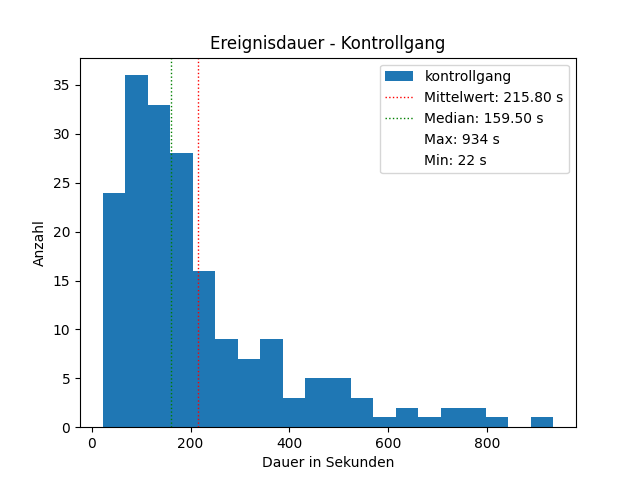
\includegraphics[width=1.1\linewidth]{img//Ereignisdauer/Auswertung Ereignisdauer kontrollgang.png}
        \caption{Kontrollgang}
        \label{fig:DauerKontroll}
    \end{subfigure}%
    \begin{subfigure}{.5\textwidth}
        \centering
        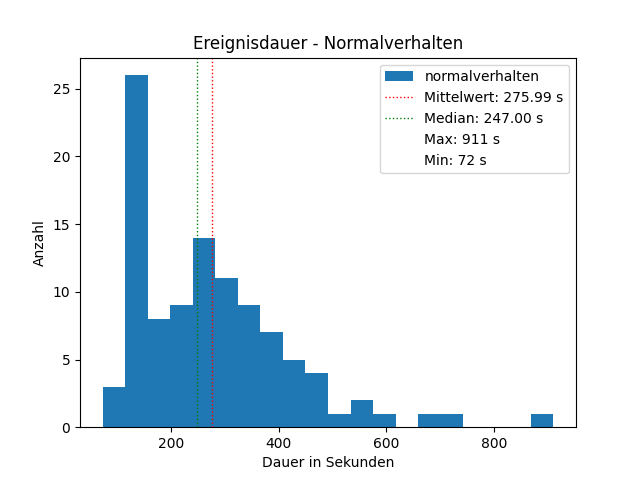
\includegraphics[width=1.1\linewidth]{img//Ereignisdauer/Auswertung Ereignisdauer normalverhalten.png}
        \caption{Normalverhalten}
        \label{fig:DauerKampf}
    \end{subfigure}
    \begin{subfigure}{.6\textwidth}
        \centering
        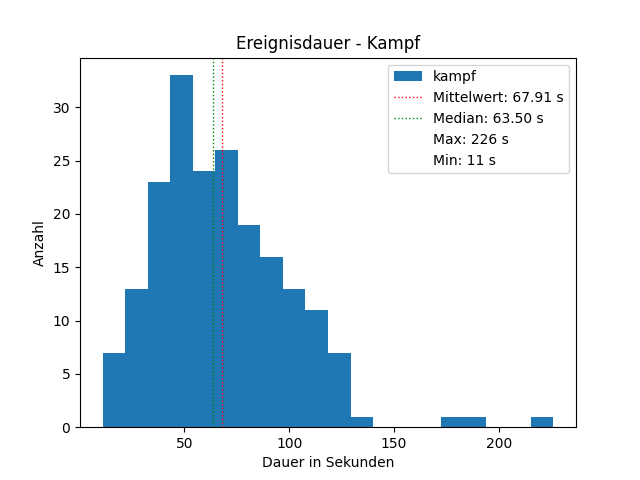
\includegraphics[width=1\linewidth]{img//Ereignisdauer/Auswertung Ereignisdauer kampf.png}
        \caption{Kampf}
        \label{fig:DauerNormal}
    \end{subfigure}
    \caption[Histogramme der zeitlichen Längen der Ereignisse im verifizierten Datensatz.]{Histogramme der zeitlichen Längen der Ereignisse im verifizierten Datensatz. (a) zeigt die Dauer der Kontrollgänge. In (b) sind die Längen des Normalverhaltens zu sehen. (c) zeigt die Kampfereignisse. Es ist jeweils der Mittelwert und der Median eingezeichnet. In der Legende sind Minmal- und Maximalwerte angegeben.}
    \label{fig:EreignisDauer}
\end{figure}

\subsection{Erstellung des Ursprungsdatensatzes}
In \autoref{fig:EreignisDauer} ist zusehen, dass die Kämpfe im Schnitt am kürzesten sind. Diese dauern meistens nur ungefähr eine Minute. Auch das kürzeste Ereignis ist ein Kampf mit 11 Sekunden. Insgesamt fällt auf, dass die unterschiedlichen Ereignisse sehr unterschiedlich Lang seien können. Kontrollgänge sind i.d.R deutlich länger als Kämpfe. Aber auch innerhalb einer Verhaltensweise kann die Länge deutlich variieren. Da die Ausgewählten Modelle die Zeitreihen der Ereignisse in Form von komprimierten Features erhalten sollen, macht diese Varianz die Vergleichbarkeit der Ereignisse kompliziert. Bezogen auf die Anwendung des Moduls zur Verhaltensklassifikation ist das herausfordernd, da das Modul nicht weis, wie Lang das aktuell abgetastete Ereignis ist und wie viele Zeitschritte er zur Erkennung von diesem komprimieren muss. \par

um dieses Problem zu lösen werden die Ereignisse zerteilt in gleich große Abschnitte. Ein Kontrollgangereignis, welches 6 Minuten geht, wird bspw. in 6 Abschnitte von jeweils einer Minute Länge geteilt. Das gleiche geschieht mit allen Ereignissen, so dass ein Datensatz entsteht, in dem alle Ereignisse die gleiche Länge haben. Für die Anwendung des Moduls zur Verhaltensklassifikation ist das Vorteilhaft, da das Modul somit feste Intervalle auswertet. Dadurch wird keine Abschätzung der Ereignisdauer benötigt. \par

Es ist zu bestimmen, welche Intervalllänge für das Modul und die Aufgabe geeignet ist. Dazu sind die Faktoren zu betrachten, die damit in einem Zusammenhang stehen. Um eine konstante lückenlose Abtastung des Stallgeschehens zu erreichen, darf der Intervall maximal so lang sein, wie die Laufzeit des Moduls. Wünschenswerter ist jedoch, dass sich die Intervalle bei der Abtastung überlappen. Ist das nicht der Fall kann es passieren, dass ein Ereignis so zerteilt wird, das die charakteristischen Merkmale in der Kompression nicht mehr deutlich werden. Überlappen sich die Intervall wird die Gefahr reduziert dass ein Ereignis nicht erkannt wird. Von der Laufzeit des Moduls ist zu diesem Zeitpunkt nur die Laufzeit des Assoziationsmoduls abschätzbar. Wie in \autoref{sec:Ergebnisse MOT} dargestellt wird. Aus diesem Grund ist genügend Puffer wichtig, um im Nachhinein keine Komplikationen durch die Laufzeit des Moduls zu erhalten. Der Puffer darf jedoch nicht zu groß sein. Ist der Intervall deutlich größer als das Ereignis selbst, verwässern die charakteristischen Merkmale bei der Komprimierung. Ist der Intervall zu klein, werden die charakteristischen Merkmale nicht deutlich in den komprimierten Features. \par

Die optimale Länge des Intervalls ist schwer zu bestimmen. Über die Laufzeiten in der Abbildung \ref{fig:EreignisDauer}, lässt sich jedoch eingrenzen mit, welcher Intervalllänge ein Funktionierendes Modul zu erwarten ist. Die minimale Ereignisdauer eines Kampfes und eines Kontrollgangs lassen sich als untere Grenze für den Intervall annehmen. Es kann sein, dass die charakteristischen Merkmale bereits mit einer kürzeren Dauer eindeutig festzustellen sind. Mit der Annahme der minimalen Ereignisdauer wird jedoch sichergestellt, die Merkmale erfasst werden. Diese ist für die Kontrollgänge länger als für Kämpfe. Das minimale Kontrollgangereignis dauert 22 Sekunden. Um einen Kontrollgang eindeutig zu erfassen, wird angenommenem, dass der Intervall mindestens 22 Sekunden umfassen muss. \par

Aus dem Mittelwert und Median der Kampfdauer lässt sich eine Eingrenzung der maximalen Intervalldauer ableiten. Die Kämpfe sind im Mittel die kürzesten Ereignisse. Der Mittelwert liegt bei 68 Sekunden und der Median bei 64 Sekunden. Die Hälfte aller Kämpfe ist somit kürzer als 64 Sekunden. Um die Erfassung der charakteristischen Merkmale von Kämpfen nicht zu verwässern, ist es sinnvoll unterhalb des Median zu bleiben. \par

Das in der Anwendung der Start eines Ereignis exakt auf den Anfang eines Intervalls fällt ist unwahrscheinlich. Um dennoch möglichst frühzeitig ein Ereignis zu erkennen, macht es Sinn einen gewissen Grad der Verwässerung zu erlauben, bei welchem die charakteristischen Merkmale dennoch sichtbar genug bleiben. Dieser wird auf 75 \% geschätzt. 75 \% des Intervalls müssen die charakteristischen Merkmale eines Ereignis beinhalten, damit dieses Erkannt werden kann. Bezogen auf die untere Grenze von 22 Sekunden bedeutet dies, dass der Intervall maximal 29 Sekunden lang seien darf, damit auch die kürzesten Kontrollgänge noch frühzeitig erkannt werden. \par

Um genügend Puffer für die Laufzeit des Moduls einzuplanen wird der Intervall auf einen Länge von 40 Sekunden gesetzt. Für einen größeren Puffer wird in Kauf genommen, dass die kürzesten Ereignisse nicht erkannt werden können. Ereignisse die kürzer als \(40 s \cdot 75 \% = 30 s\) sind, werden so nicht erkannt. Die Tabelle \ref{tab:DataNachIntervall} zeigt, wie sich das auf die Menge der Ereignisse auswirkt, die genutzt werden können.\par

\begin{table}[ht]
    \centering
    \caption{Zusammensetzung des Datensatzes nach festlegen des Intervalls.}
    \begin{tabular}{|l|r|r|r|}
    \hline
        Verhaltensweise & Anzahl & Anteil & Veränderung\\
    \hline
        Normalverhalten & 103 & 22 \% & -0 \%\\
        Kontrollgang & 186 & 40 \% & +1 \%\\
        Kampf & 175 & 39 \% & -11 \%\\
    \hline
    \hline
        Gesamt & 470 & 100 \% & -5 \% \\
    \hline
    \end{tabular}
    \label{tab:DataNachIntervall}
\end{table}

Da nun der Intervall feststeht können die Ereignisse auf feste Längen aufgeteilt werden. Um \gls{Leakage} zu vermeiden geschieht dies ohne Überlappung. Damit das Modell lernen kann, ein Ereignis zu erkennen, welches nicht die vollen 40 Sekunden umfasst, werden Proben benötigt, in welche das Ereignis in einer Länge von 30 Sekunden bis 40 Sekunden stattfindet. Dazu wird die Startzeitpunkte und die Endzeitpunkte der Ereignisse auf die nächsten vollen 10 Sekunden gerundet. Die Startzeitpunkte werden abgerundet und die Endzeitpunkte werden aufgerundet. Der Startzeitpunkt \(13:00:57\) würde dem entsprechend auf \(13:00:50\) vorgezogen werden und der Endzeitpunkt \(13:02:17\) verschiebt sich nach hinten auf \(13:02:20\). \par

In der Tabelle \ref{tab:DataNachIntervall} ist zu sehen, dass die Gesamtanzahl der Ereignisse dadurch um 5 \% reduziert wird. Am negativsten wirkt sich der Intervall auf die Kampfereignisse aus. Diese werden um 11 \% reduziert. Da die Kampfereignisse vom großen Interesse sind, ist dieser Datenverlust beträchtlich. Er wird jedoch in Kauf genommen, da die restlichen Kampfereignisse somit sicher die charakteristischen Merkmale beinhalten und das in einer Intensität, das dass Modul diese sich er erkennen können sollte. Es sollte sich positiv auf die Datenqualität auswirken. \par

Mit diesen Überlegungen können die Ereignisse zerteil werden. In der Tabelle \ref{tab:DatasetSplit} ist zu sehen welche Datenmengen sich dadurch ergeben. 

\begin{table}[ht]
    \centering
    \caption{Zusammensetzung des Datensatzes nach der Aufteilung gemäß des Intervalls.}
    \begin{tabular}{|l|r|r|r|}
    \hline
        Verhaltensweise & Anzahl & Anteil \\
    \hline
        Normalverhalten & 683 & 35 \% \\
        Kontrollgang & 969 & 50 \% \\
        Kampf & 290 & 15 \% \\
    \hline
    \hline
        Gesamt & 1942 & 100 \%\\
    \hline
    \end{tabular}
    \label{tab:DatasetSplit}
\end{table}

Bei der Feature-Extraktion und Konstruktion viel auf, dass die Detektion im Stall erst ab dem 19.04.2021 stabil lief. Die Detektionsdatensätze davor beinhalten viele Einträge in denen nichts detektiert wurde. Aus den Ereignissen in diesem Zeitraum sind keine Features extrahierbar, weshalb sie nicht für den Aufbau des Modells verwendet werden können. Die Tabelle \ref{tab:DatasetFeatExtr} zeigt die Auswirkungen auf die Datenmenge.

\begin{table}[ht]
    \centering
    \caption{Zusammensetzung des Datensatzes nach der Aufteilung gemäß des Intervalls.}
    \begin{tabular}{|l|r|r|r|}
    \hline
        Verhaltensweise & Anzahl & Anteil & Veränderung\\
    \hline
        Normalverhalten & 572 & 40 \% & -16 \%\\
        Kontrollgang & 868 & 61 \% & -10 \%\\
        Kampf & 220 & 15 \% & -24 \%\\
    \hline
    \hline
        Gesamt & 1660 & 100 \% & -15 \% \\
    \hline
    \end{tabular}
    \label{tab:DatasetFeatExtr}
\end{table}


\subsection{Diskussion der Datenmenge}
Vorteilhaft ist, dass sich durch die Aufteilung gemäß der Intervalle die Anzahl der Proben deutlich erhöht hat. Für \gls{ML} kann die Datenmenge entscheidend sein. Mit 1660 Ereignissen ist die Datenmenge im Kontext des maschinellen Lernens relativ klein. Hinzukommt, dass der Datensatz unbalanciert ist. Der Anteil der Kämpfe ist deutlich niedriger, als der Anteil der anderen beiden Verhaltensweisen. Damit war zu rechnen, da die Kontrollgänge und das Normalverhalten im Schnitt deutlich länger sind, als Kämpfe, wie in den Histogrammen in \autoref{fig:EreignisDauer} zu sehen ist. Durch die Einteilung in die Intervalle, entstehen aus einem Kontrollgang somit mehr Proben, als aus einem Kampfereignis. Um mit dem Datensatz ein Modell zu trainieren ist es Ratsam dieses mittels Undersampling auszubalancieren (\autoref{sec:Datensätze ML}). Dadurch reduziert sich die effektiv nutzbare Datenmenge wie in Tabelle \ref{tab:DataNachBalance} dargestellt.

\begin{table}[ht]
    \centering
    \caption{Zusammensetzung des Datensatzes nach festlegen des Intervalls.}
    \begin{tabular}{|l|r|r|r|}
    \hline
        Verhaltensweise & Anzahl & Anteil & Veränderung\\
    \hline
        Normalverhalten & 220 & 33 \% & -62 \%\\
        Kontrollgang & 220 & 33 \% & -75 \%\\
        Kampf & 220 & 33 \% & -0 \%\\
    \hline
    \hline
        Gesamt & 660 & 100 \% & -60 \% \\
    \hline
    \end{tabular}
    \label{tab:DataNachBalance}
\end{table}

Für maschinelles Lernen ist dies eine sehr geringe Datenmenge. Bei dem Aufbau des Modells besteht große Gefahr für Overfitting. Durch die Verifizierung der Ereignisse besteht jedoch die Hoffnung, dass die Qualität der Daten hoch ist. Das erhöht die Chancen ein funktionierendes Modell aufzubauen. \par

Der Datensatz besitzt einen Bias durch geringe Varianz. Die Daten stammen aus einem sehr begrenzten Zeitraum, aus nur einem Mastdurchlauf. Die Daten entstammen einem Zeitraum von zwei Monaten vom 19.04.2021 bis zum 18.06.2021 \todo{Daten kontrollieren}. Es sind nur zwei Kameras ausgewertet worden, die Kameras mit den IDs 3 und 5. Dadurch besteht auch hier ein Bias in Bezug auf den Stallbereich. Diese Voreingenommenheiten können dafür sorgen, dass das Modell schlecht anwendbar auf beliebige Stallbereiche ist. \par

Zusammenfassend lässt sich sagen, dass die Datenlage unvorteilhaft ist, um ein Modell aufzubauen, welches gut generalisieren soll. Die Datenqualität kann dem möglicherweise Entgegenwirken. Das bewusst machen der Schwächen der Datengrundlage, kann dazu genutzt werden, um im Featureengineering und der Modellkonfiguration Gegenmaßnahmen zu ergreifen. Gerade im Bezug auf die Vermeidung von Overfitting.